\clearpage

\section{Ideal Amplifier}

\maketitle

This block has one input signal and one output signal both corresponding to electrical signals. The output signal is a perfect amplification of the input signal.


\subsection*{Input Parameters}


\begin{table}[h]
	\centering
	\begin{tabular}{|c|c|c|c|c}
		\cline{1-4}
		\textbf{Parameter} & \textbf{Type} &\textbf{Values} &   \textbf{Default}& \\ \cline{1-4}
		gain 	   		 & double & any 	& $1 \times 10^{4}$& \\ \cline{1-4} \cline{1-4}
	\end{tabular}
	\caption{Ideal Amplifier input parameters}
	\label{table:idealamp_in_par}
\end{table}


\subsection*{Methods}
 
IdealAmplifier() {}
\bigbreak
IdealAmplifier(vector<Signal *> \&InputSig, vector<Signal *> \&OutputSig) :Block(InputSig, OutputSig){};
\bigbreak
void initialize(void);
\bigbreak
bool runBlock(void);
\bigbreak
void setGain(double ga) { gain = ga; }
\bigbreak
double getGain() { return gain; }


\subsection*{Functional description}

The output signal is the product of the input signal with the parameter \textit{gain}. 

\pagebreak

\subsection*{Input Signals}

\subparagraph*{Number:} 1

\subparagraph*{Type:} Electrical (TimeContinuousAmplitudeContinuousReal)

\subsection*{Output Signals}

\subparagraph*{Number:} 1

\subparagraph*{Type:} Electrical (TimeContinuousAmplitudeContinuousReal)

\subsection*{Examples} 

%\begin{figure}[h]
%	\centering
%	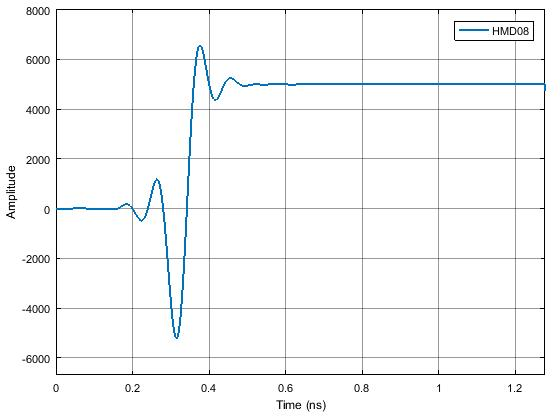
\includegraphics[width=\textwidth]{../homodyne_receiver/figures/TIAmplifier_output}
%	\caption{Example of the output signal of the amplifier block for a binary sequence 01. Note the scale of the y axis in comparison to the one in the output signal of the photodiode. The shape of the signal is the same as expected}\label{IdealAmplifier_output}
%\end{figure}

\subsection*{Sugestions for future improvement}

